%!TEX TS-program = xelatex
\documentclass[10pt]{article}
\usepackage{amsmath,amssymb,amsfonts} % Typical maths resource packages
\usepackage{float}
\usepackage{graphics}                 % Packages to allow inclusion of graphics
\usepackage{color}                    % For creating coloured text and background
\usepackage{hyperref}
\usepackage{graphicx}                 % For Figures
\usepackage{xepersian}                % For Persian language support


\settextfont{XB Niloofar.ttf}
\hypersetup{
	colorlinks=true,
	linkcolor=black,
	filecolor=magenta,      
	urlcolor=cyan,
	pdftitle={Overleaf Example},
	pdfpagemode=FullScreen,
}

\begin{document}

\title{بسم اللّه الرحمن الرحیم
	\\[25pt]	پروژه پایانی پردازش زبان طبیعی
}
\author{غزاله محمودی}

\date{\today}
\maketitle
\newpage

\tableofcontents
\newpage

\listoffigures
\newpage

\listoftables
\newpage
	
\section{ 
	\lr{word2vec}
}
در این بخش قصد داریم با استفاده از ماژول gensim بردار
\lr{word 2 vec}
  را برای هر کلمه حساب کنیم.
ابتدا لازم است دیتاست را برای استفاده آماده کنیم. به کمک pandas و نظرات موجود را استخراج می کنیم. در نهایت DataFrame به صورت زیر حاصل می شود.


در ادامه به ازای تمام نظرات(جملات) موجود در دیتاست کلمات موجود در آن ها را استخراج می کنیم. این کار با استفاده از tokenizer ماژول HAZM انجام می دهیم. 


برای به دست آوردن word2vev به کمک Gensim تعدادی پارامتر قابل تنظیم دارد که در ادامه به بررسی آن ها می پردازم.

\begin{itemize}
	\item Size 
	
	این پارامتر تعیین کننده سایز vector برای نمایش هر word یا token است. هر چه دیتاست محدود تر و کوچکتر باشد این عدد نیز کوچک تر در نظر گرفته می شود و هر چه دیتاست بزرگتر باشد(کلمات unique بیشتری داشته باشد) باید اندازه vector بزرگتر در نظر گرفته شود. تجربه نشان داده اندازه بین 100 تا 150 برای دیتاست های بزرگ مقدار مناسبی است.
	
	\item Windows 
	
	این پارامتر تعیین کننده بیشترین فاصله مابین کلمه اصلی و همسایه های آن می باشد.از لحاظ تئوری هر چه این سایز کوچکتر باشد کلماتی که بیشتر ارتباط را به یکدیگر دارند به عنوان خروجی برمی گرداند. اگر تعداد داده به اندازه کافی بزرگ باشد سایز پنجره اهمیت زیادی ندارد اما باید این نکته را در نظر گرفت که این سایز نباید خیلی بزرگ یا بیش از حد کوچک باشد. اگر درباره انتخاب آن اطمینان نداریم بهتر است از مقدار پیش فرض استفاده کنیم.
	
	
	\item \lr{Min count}
	
	این پارامتر حداقل تکرار کلمه در دیتاست را نشان می دهد که در صورتی که کلمه ای به این تعداد تکرار شود در
	\lr{word embedding}
	 مورد توجه قرار می گیرد و در غیر این صورت کنار گذاشته می شود. تعیین این عدد در دیتاست های بزرگ برای کنار گذاشتن کلمات کم اهمیت که غالبا کم تکرار می شوند مناسب است. همچنین در مصرف بهینه مموری و حافظه هم تاثیر دارد.
	
	 
	\item Workers
	
	این پارامتر تعداد thread هایی که در عملیات اجرا مورد استفاده قرار می گیرد را مشخص می کند. برای عملیات بهینه سازی و افزایش سرعت اجرا در سیستم هایی که قابلیت پردازش موازی دارند.
	
	 
	\item Iter
	
	تعداد epoch یا دفعاتی که الگوریتم اجرا می شود و مدل آموزش می بیند.
	 
	\item seed 
	
	برای مقدار دهی رندوم اولیه استفاده می شود.
\end{itemize}
	
	\begin{figure}[ht!]
		\centering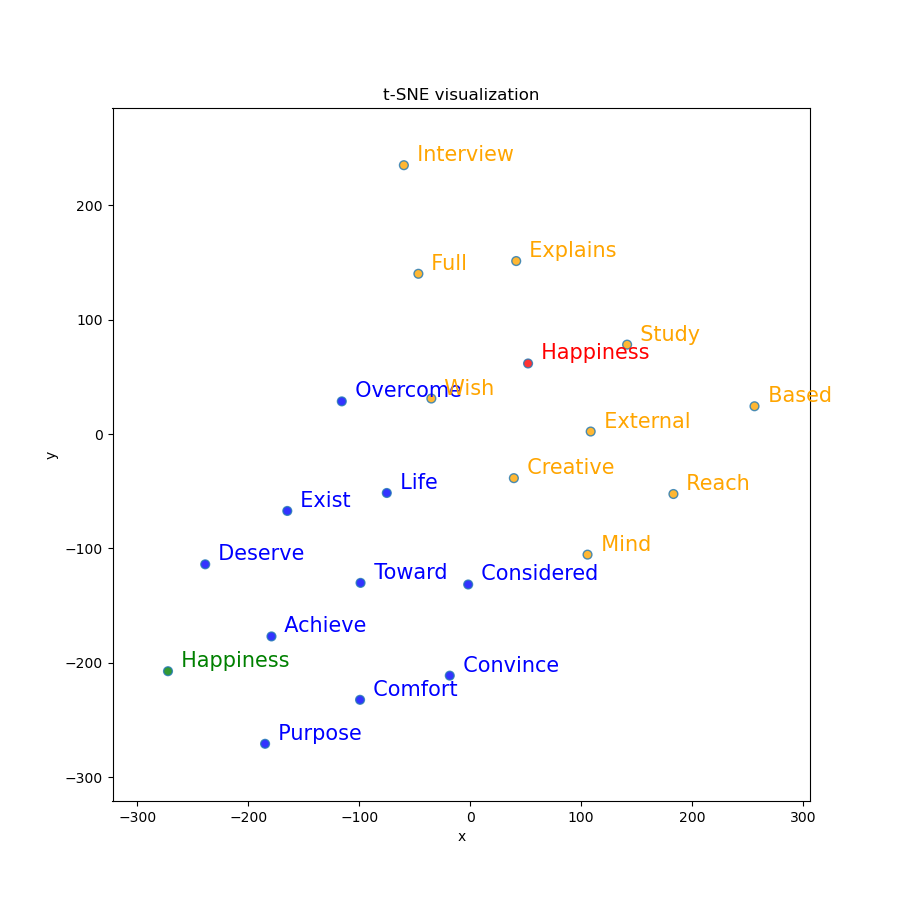
\includegraphics[width=\linewidth]{../reports/word_vectors_common_happiness.png}
		\caption{شبکه 
			\lr{language model}}
		\label{word2vec-1}
	\end{figure}

	\begin{figure}[ht!]
	\centering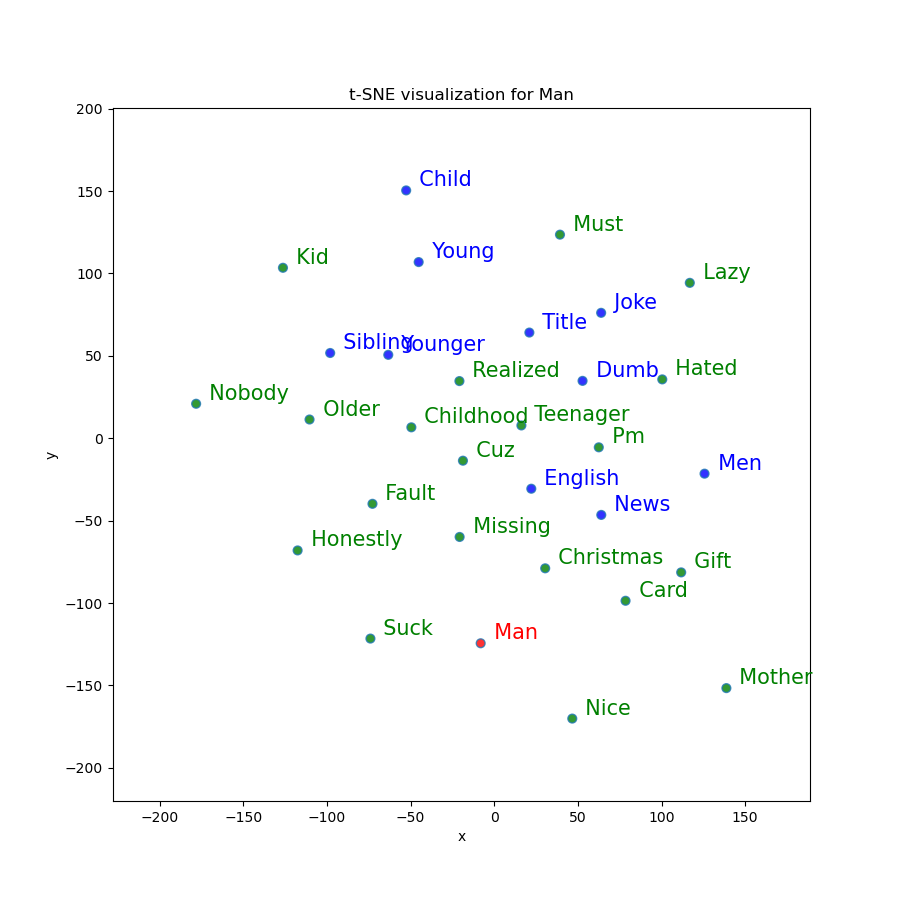
\includegraphics[width=\linewidth]{../reports/_word_vectors_common_man.png}
	\caption{شبکه 
		\lr{language model}}
	\label{word2vec-2}
	\end{figure}

\newpage
\section{
	\lr{tokenization}
}

\newpage
\section{
	\lr{parsing}
}

\newpage
\section{
	\lr{language model}}
	در این بخش برای آموزش 
	\lr{language model}
	ابتدا داده تمیز را به صورت مناسب آماده می‌کنیم. سپس به ازای هر کدام از دسته‌های 
	\lr{depresion}
	و
	\lr{happiness}
	داده را به شبکه داده تا مدل زبانی آموزش ببیند. در معماری تعریف شده ایتدا یک لایه 
	\lr{embedding}
	قرار داده شده و در ادامه لایه 
	\lr{LSTM}
	با 
	\lr{100 hidden state}
	قرار دارد. لایه دیگری
	\lr{bidirectional LSTM}
	و در ادامه یک لایه dense قرار دارد. لایه انتهایی یک لایه dense یا تابع فعال‌سازی softmax می‌باشد که به تعداد همه کلمات موجود نورون دارد. در این لایه به ازای ورودی شبکه مشخص می‌شود چه کلمه باید بعد از عبارت ورودی شبکه بیاید.
	مدل تعریف شده به صورت شکل\ref{lm}
	می‌باشد. دقت و loss برای کلاس‌های مختلف به صورت شکل\ref{lm_dep} و شکل\ref{lm_hap} است.
	
	\begin{figure}[ht!]
		\centering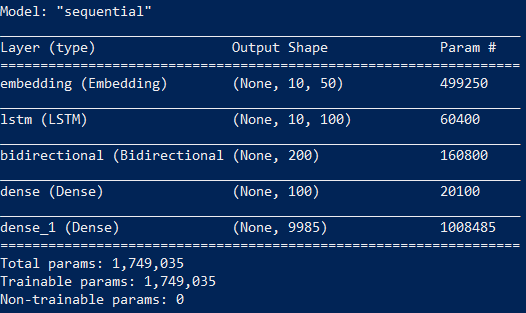
\includegraphics[width=\linewidth]{../reports/lm_model.png}
		\caption{شبکه 
			\lr{language model}}
		\label{lm}
	\end{figure}
	
	
	\begin{figure}[ht!]
		\centering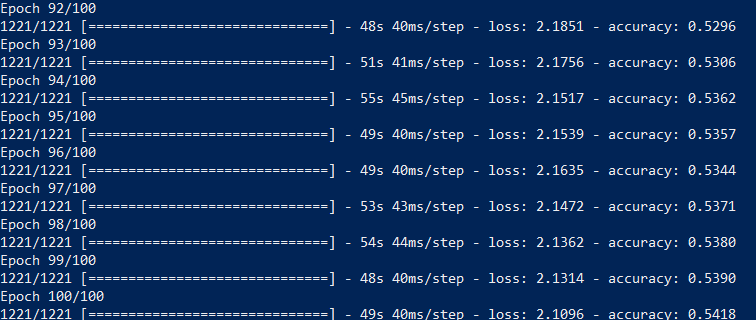
\includegraphics[width=\linewidth]{../reports/lm_dep.png}
		\caption{ 
			\lr{LSTM accuracy and Loss language model on class depression}}
		\label{lm_dep}
	\end{figure}

	\begin{figure}[ht!]
		\centering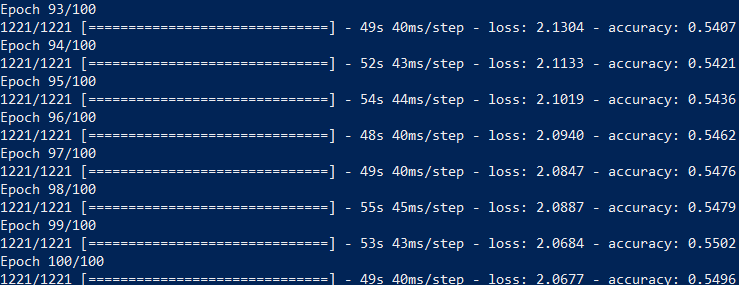
\includegraphics[width=\linewidth]{../reports/lm_hap.png}
		\caption{
			\lr{LSTM accuracy and Loss language model on class happiness}}
		\label{lm_hap}
	\end{figure}


\begin{itemize}
	\item happiness
	
	\lr{take break outside lunch feel like everyone office hate think boring
		since forced office romantic vacation friend friend whole money laying}
	
	\item happiness
	 
	\lr{kill prayed god make accident happen year old relationship family know
		remember im told reminds friend something really eventually wa using}
	
	\item happiness
	
	\lr{i feel so .. like losing grow shell remember hate suck suck fucked cant}
	
	\item depression
	
	\lr{i feel so .. like edgy movie mind hold supportive defense trash sea man}
\end{itemize}

	
\newpage
\section{
	\lr{finu tuning}
}

\subsection{\lr{language model}}
در این بخش با توجه به مطالعات انجام شده بر روی مدل‌های
\lr{GPT2}
 در 
\lr{language model}
و کیفیت خروجی مدل برای این تسک، از
\lr{distilgpt2}
به عنوان مدل pretrain استفاده کرده و مدل را بر دیتاست موجود finetune کردم.

برای اجرا این بخش کافیست
\lr{python3 fine\_tuning.py GPT2}
را اجرا کنید.
به ازای هر کدام از کلاس‌های 
\lr{depresion}
و
\lr{happiness}
مدل را finetune کرده و وزن‌های حاصله به صورت اتوماتیک در
\lr{models/depressionGPT2\_lm}
و
\lr{mosels/happinessGPT2\_lm}
ذخیره می‌شوند. همچنین log در حین اجرا در 
\lr{logs/fine\_tuning\_GPT2.log}
قابل مشاهده هست. نمودار تغییرات  
\lr{loss}
مدل در زمان finetune برای کلاس
\lr{depression}
 به صورت شکل\ref{GPT_dep}
 و برای کلاس
 \lr{happiness}
به صورت شکل\ref{GPT_hap}
می‌باشد.
	\begin{figure}[H]
		\centering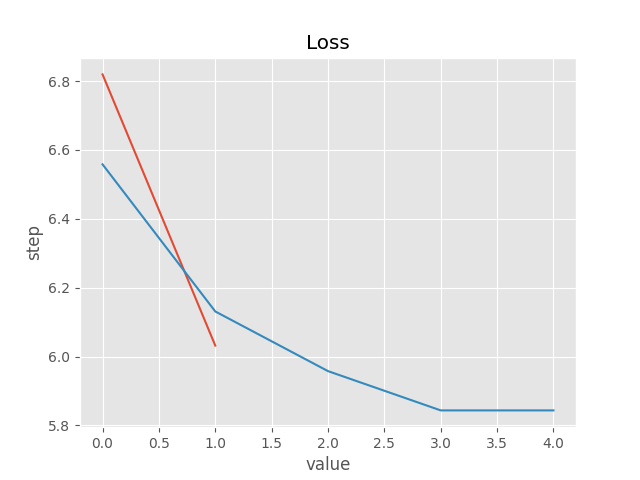
\includegraphics[width=\linewidth]{../reports/loss_history_GPT2_depression.png}
		\caption{ 
			\lr{distilgpt2 Loss language model on class depression}}
		\label{GPT_dep}
	\end{figure}
	
		\begin{figure}[H]
		\centering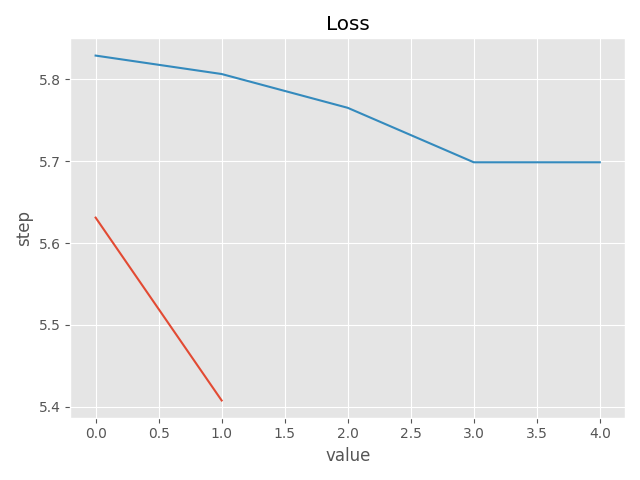
\includegraphics[width=\linewidth]{../reports/loss_history_GPT2_happiness.png}
		\caption{ 
			\lr{distilgpt2 Loss language model on class happiness}}
		\label{GPT_hap}
	\end{figure}


جملات تولید شده با مدل از قبل آموزش دیده
\lr{distilgpt2}
بسیار با کیفیت‌ترو معنی‌دارتر از جملات تولید شده در قسمت قبل می‌باشد.
به ازای هر کدام از کلاس‌ها دو جمله تولید شده که به صورت زیر می‌باشد. نوشته به رنگ آبی توسط مدل تولید شده است.

\begin{itemize}
	\item happiness
	
	\lr{Hi, we have created a success forum for
		since forced office romantic vacation friend friend whole money laying}
	
	
	\item happiness
	
	\lr{Hi, we have created a success forum for}
	\lr{people interested interested    know going want succeed going want fail people want know go past time never successful people want know go past time know succeeding people want know go past time life lived time lived past moment}\color{blue}\\
	
	
	\item happiness
	
	\lr{I'm so depressed. I have nothing to live
		remember im told reminds friend something really eventually wa using}
	
	
	\item depression
	
	\lr{I'm so depressed. I have nothing to live}
	\lr{like edgy movie mind hold supportive defense trash sea man}\color{blue}
\end{itemize}

\subsection{\lr{classification}}
در بخش دوم مدل 
\lr{bert-base-uncased}
از قبل آموزش دیده را برای classification داده‌ها بر روی داده‌های موجود finetune می‌کنیم. 
برای اجرا این بخش کافیست
\lr{python3 fine\_tuning.py Bert}
را اجرا کرد. وزن‌های مدل finetune شده در 
\lr{models/bert\_classification\_lm}
ذخیره می‌شوند. همچنین log در حین اجرا در 
\lr{logs/fine\_tuning\_Bert.log}
می‌باشد. نمودار تغییرات loss در شکل\ref{bert}
قابل مشاهده است.

\begin{figure}[ht!]
	\centering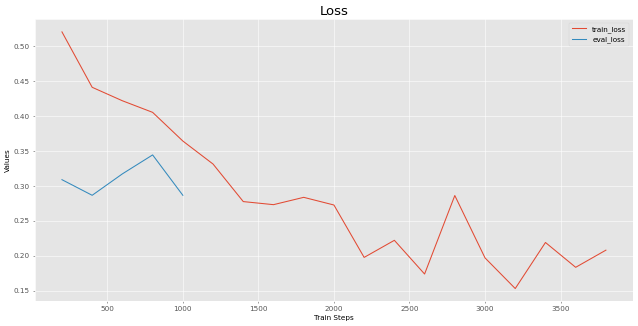
\includegraphics[width=\linewidth]{../reports/loss_history_Bert.png}
	\caption{ 
		\lr{bert-base-uncased Loss classification}}
	\label{bert}
\end{figure}


\newpage

\section{منابع}

\begin{flushleft}
	\url{https://radimrehurek.com/gensim/models/word2vec.html}
	%\url{https://colab.research.google.com/github/google/sentencepiece/blob/master/python/sentencepiece\_python\_module\_example.ipynb#scrollTo=T9BDzLVkUFT4
	\url{https://www.philschmid.de/fine-tune-a-non-english-gpt-2-model-with-huggingface}
	\url{https://machinelearningmastery.com/how-to-develop-a-word-level-neural-language-model-in-keras/}
	\url{https://gmihaila.github.io/tutorial_notebooks/pretrain_transformers_pytorch/}
\end{flushleft}

\end{document}